\subsection{Alpha and Beta Decomposition}
\label{Subsection:AlphaBeta}

A currency pair moves on its own. An agent that is long a pair which happens to rise will show a profit that has nothing to do with the policy it learned, and an agent that is short a pair which happens to fall will show the same. Total return cannot tell the two apart, so the results are decomposed into the part explained by the market and the part that is not.

For each pair the yearly return of the model is regressed on the yearly move of the pair itself, over the eleven years from 2015 to 2025. Writing $r_i$ for the model return in year $i$ and $m_i$ for the market move in the same year, ordinary least squares gives

\begin{equation}
\beta = \frac{\sum_i (m_i - \bar{m})(r_i - \bar{r})}{\sum_i (m_i - \bar{m})^2}, \qquad \alpha = \bar{r} - \beta \bar{m}
\label{Equation:AlphaBeta}
\end{equation}

$\beta$ is how much of the market's movement the model carries, and $\alpha$ is the average yearly return left once that exposure is removed. The mean return then splits into an active part and a passive one:

\begin{equation}
\bar{r} = \underbrace{\alpha}_{\text{policy}} + \underbrace{\beta \bar{m}}_{\text{market exposure}}
\label{Equation:AlphaDecomposition}
\end{equation}

Yearly rather than daily returns are used for a specific reason. The agents hold positions for days to weeks and act once per day, so a daily regression would measure how the model tracks the market within a holding period rather than whether it chose the right direction over the horizon it trades. Eleven yearly observations is a small sample and the individual coefficients carry wide uncertainty; what the decomposition supports is the separation of pairs into groups, not a precise value for any one of them.

Table~\ref{Tables:AlphaBeta} gives both terms. Six of the seven pairs have positive alpha, and the seven fall into three clear groups.

\begin{table}[htb!]
\centering
\footnotesize
\begin{tabular}{@{}lrrrrl@{}}
\toprule
\textbf{Pair} & \textbf{Beta} & \textbf{Alpha (\%/yr)} & \textbf{Beta Return (\%/yr)} & \textbf{Mean (\%/yr)} & \textbf{Reading} \\
\midrule
AUD/USD & $-2.013$ & $+4.96$ & $+3.22$ & $+8.18$ & Policy plus leveraged trend \\
EUR/USD & $+0.266$ & $+6.62$ & $+0.01$ & $+6.63$ & Policy, no market exposure \\
GBP/USD & $-0.054$ & $+11.64$ & $+0.06$ & $+11.70$ & Policy, no market exposure \\
NZD/USD & $-0.708$ & $+2.79$ & $+1.83$ & $+4.62$ & Policy plus leveraged trend \\
USD/CAD & $+2.393$ & $+10.02$ & $+4.21$ & $+14.23$ & Policy plus leveraged trend \\
USD/CHF & $-0.082$ & $+3.91$ & $+0.16$ & $+4.07$ & Policy, no market exposure \\
USD/JPY & $+1.012$ & $-1.08$ & $+2.64$ & $+1.57$ & No policy; the model is the market \\
\bottomrule
\end{tabular}
\caption{Decomposition of Equation~\ref{Equation:AlphaDecomposition}, from the yearly regression of Equation~\ref{Equation:AlphaBeta} over 2015 to 2025. Alpha is the return attributable to the policy and the beta return is the part explained by the pair's own movement. The two sum to the mean yearly return.}
\label{Tables:AlphaBeta}
\end{table}

\textbf{Three pairs carry almost no market exposure.} GBP/USD, EUR/USD and USD/CHF have betas of $-0.054$, $+0.266$ and $-0.082$, and their market exposure contributes $0.06$, $0.01$ and $0.16$ percentage points per year respectively. For GBP/USD, $11.64$ of its $11.70$ points per year are policy. These are the results that would survive a change in market direction, because there is almost no direction in them to change.

\textbf{Three pairs combine policy with leveraged exposure.} USD/CAD at $+2.393$, AUD/USD at $-2.013$ and NZD/USD at $-0.708$ all carry their market at meaningful size, two of them at more than twice. Their alpha is positive in every case, so there is skill on top, but between a fifth and two fifths of what they earned came from the market moving the way their exposure was pointed. USD/CAD is the clearest example: $4.21$ of its $14.23$ points per year came from the pair rising while the agent was net long. Had the Canadian Dollar strengthened over the decade instead, that component would have been a loss of similar size, and the reported $+226.6\%$ would look very different.

Figure~\ref{Figure:AlphaBeta} plots the seven together, and the three groups separate clearly.

\textbf{One pair has no policy at all.} USD/JPY has a beta of $+1.012$ and a correlation of $+0.946$ with its own market, and its alpha is $-1.08\%$ per year, the only negative figure in the table. It is examined in Section~\ref{Subsection:NegativeResult}.

\begin{figure}[htb!]
\centering
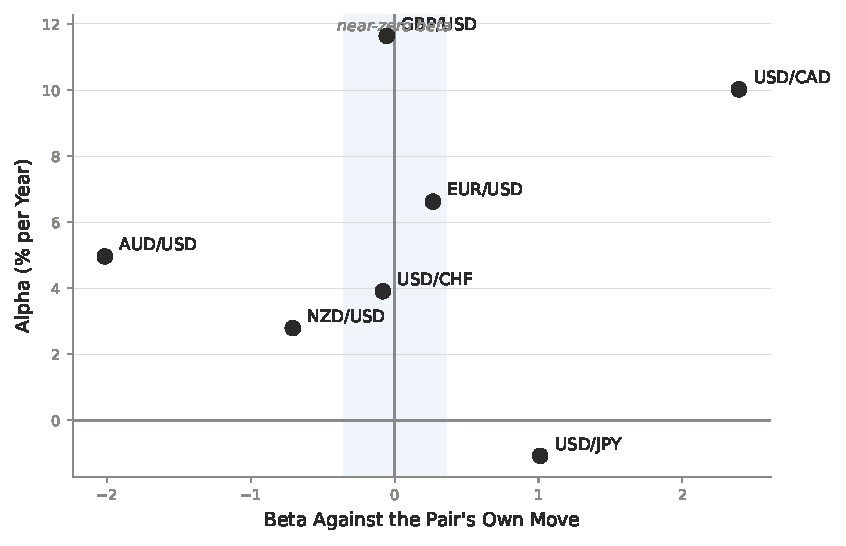
\includegraphics[width=0.82\textwidth]{Images/AlphaBeta.pdf}
\caption{Alpha against beta for the seven agents. Points inside the shaded band carry almost no market exposure, so their return is attributable to the policy. USD/JPY sits at a beta of one with negative alpha, which is the signature of a model that has reproduced its own market.}
\label{Figure:AlphaBeta}
\end{figure}

The method was checked before it was applied. Running the same regression on the model delivered by the preceding campaign reproduces its recorded figures exactly, a correlation of $+0.115$, a beta of $+0.130$ and an alpha of $+3.11\%$ per year, which confirms that the decomposition here is computed the same way as the one it is compared against.

This decomposition is reported ahead of total return for a reason that matters to how the whole section should be read. The choice of which model to publish was made from a pool of candidates, and any measure that the choice was made on is inflated by that choice. Return is such a measure. Beta is not: it describes how a policy behaves against its market, and a model cannot be selected into a low beta by luck in the way it can be selected into a high return. A large alpha with a beta near zero is therefore a stronger claim than a large return, and it is the claim this work leads with.